\subsection{Технологии визуализации результатов расчета}
\label{sec:1d}

Построение равновесной пространственной конфигурации для нанокластера
предполагает нахождение координат всех атомов кластера. Так как количество
атомов в кластере может быть достаточно большим, то необходимо визуальное
представление полученной пространственной конфигурации для помощи в последующих
исследованиях этой конфигурации. Для визуализации результатов были опробованы
два инструмента: библиотека для построения графиков DISLIN, а также
молекулярный редактор и визуализатор Avogadro.

% TODO: Insert links to tools websites to literature
DISLIN является бесплатной кросс-платформенной высокоуровневой библиотекой для
построения графиков, доступной для нескольких языков программирования (C,
Fortran, Java, Ruby, Python).  Библиотека предоставляет небольшое количество
функций непосредственно построения графиков с коротким списком параметров, а
также большое количество функций для детальной настройки различных параметров
отображения графиков.

Пример графика, построенного с помощью библиотеки DISLIN во время изучения её 
возможностей, показан на рис. \ref{DISLIN_picture}. Преимуществами библиотеки
являются простой и понятный интерфейс прикладного программирования, а также
большое количество поддерживаемых графических форматов для вывода результатов,
как векторных, так и растровых.

\begin{figure}[ht!]
\centering
  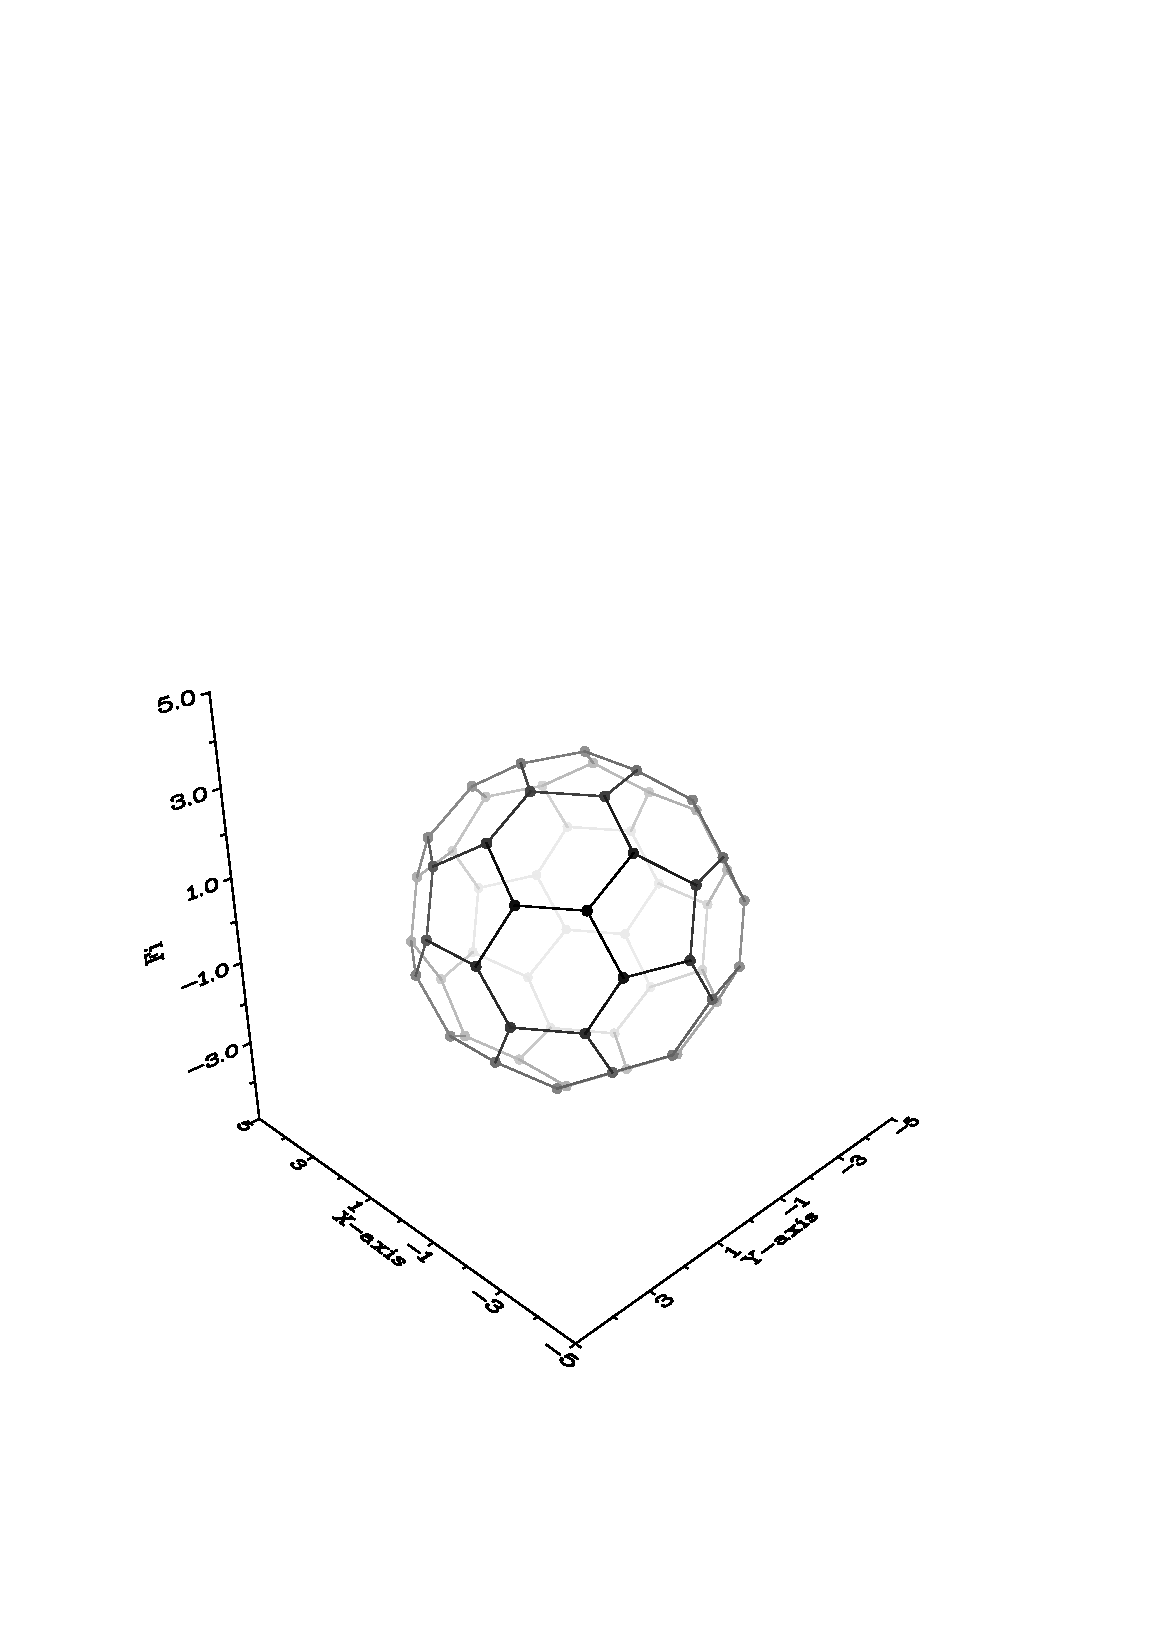
\includegraphics[trim=30 120 30 330, clip, width=0.8\textwidth]{./FIGs/DISLIN_fullerene.pdf}
\caption{Фуллерен $C_{60}$, построенный с помощью библиотеки DISLIN}
\label{DISLIN_picture}
\end{figure}

Вторым рассмотренным вариантом для визуализации результатов является молекулярный
редактор и визуализатор Avogadro. Avogadro является открытым и кросс-платформенным
программным обеспечением. Он позволяет моделировать различные химические
соединения, используя графический редактор. В качестве формата файлов для хранения
построенных моделей используется формат CML (Chemistry markup language).

Для создания и редактирования формата CML из прикладной программы существует библиотека
Open Babel. Open Babel представляет собой открытый набор утилит и библиотек для работы с
химическими данными, представленными в различных форматах. Используя библиотеку Open Babel
возможно в том числе манипулировать данными в формате CML, не вдаваясь в подробности
реализации хранения данных, а работая с такими высокоуровневыми абстракциями как молекулы и
химические связи. Пример визуального отображения модели фуллерена $C_{60}$, хранящейся в формате
CML и открытой для редактирования в приложении Avogadro представлен на рис. \ref{Avogadro_screenshot}.

\begin{figure}[ht!]
\centering
  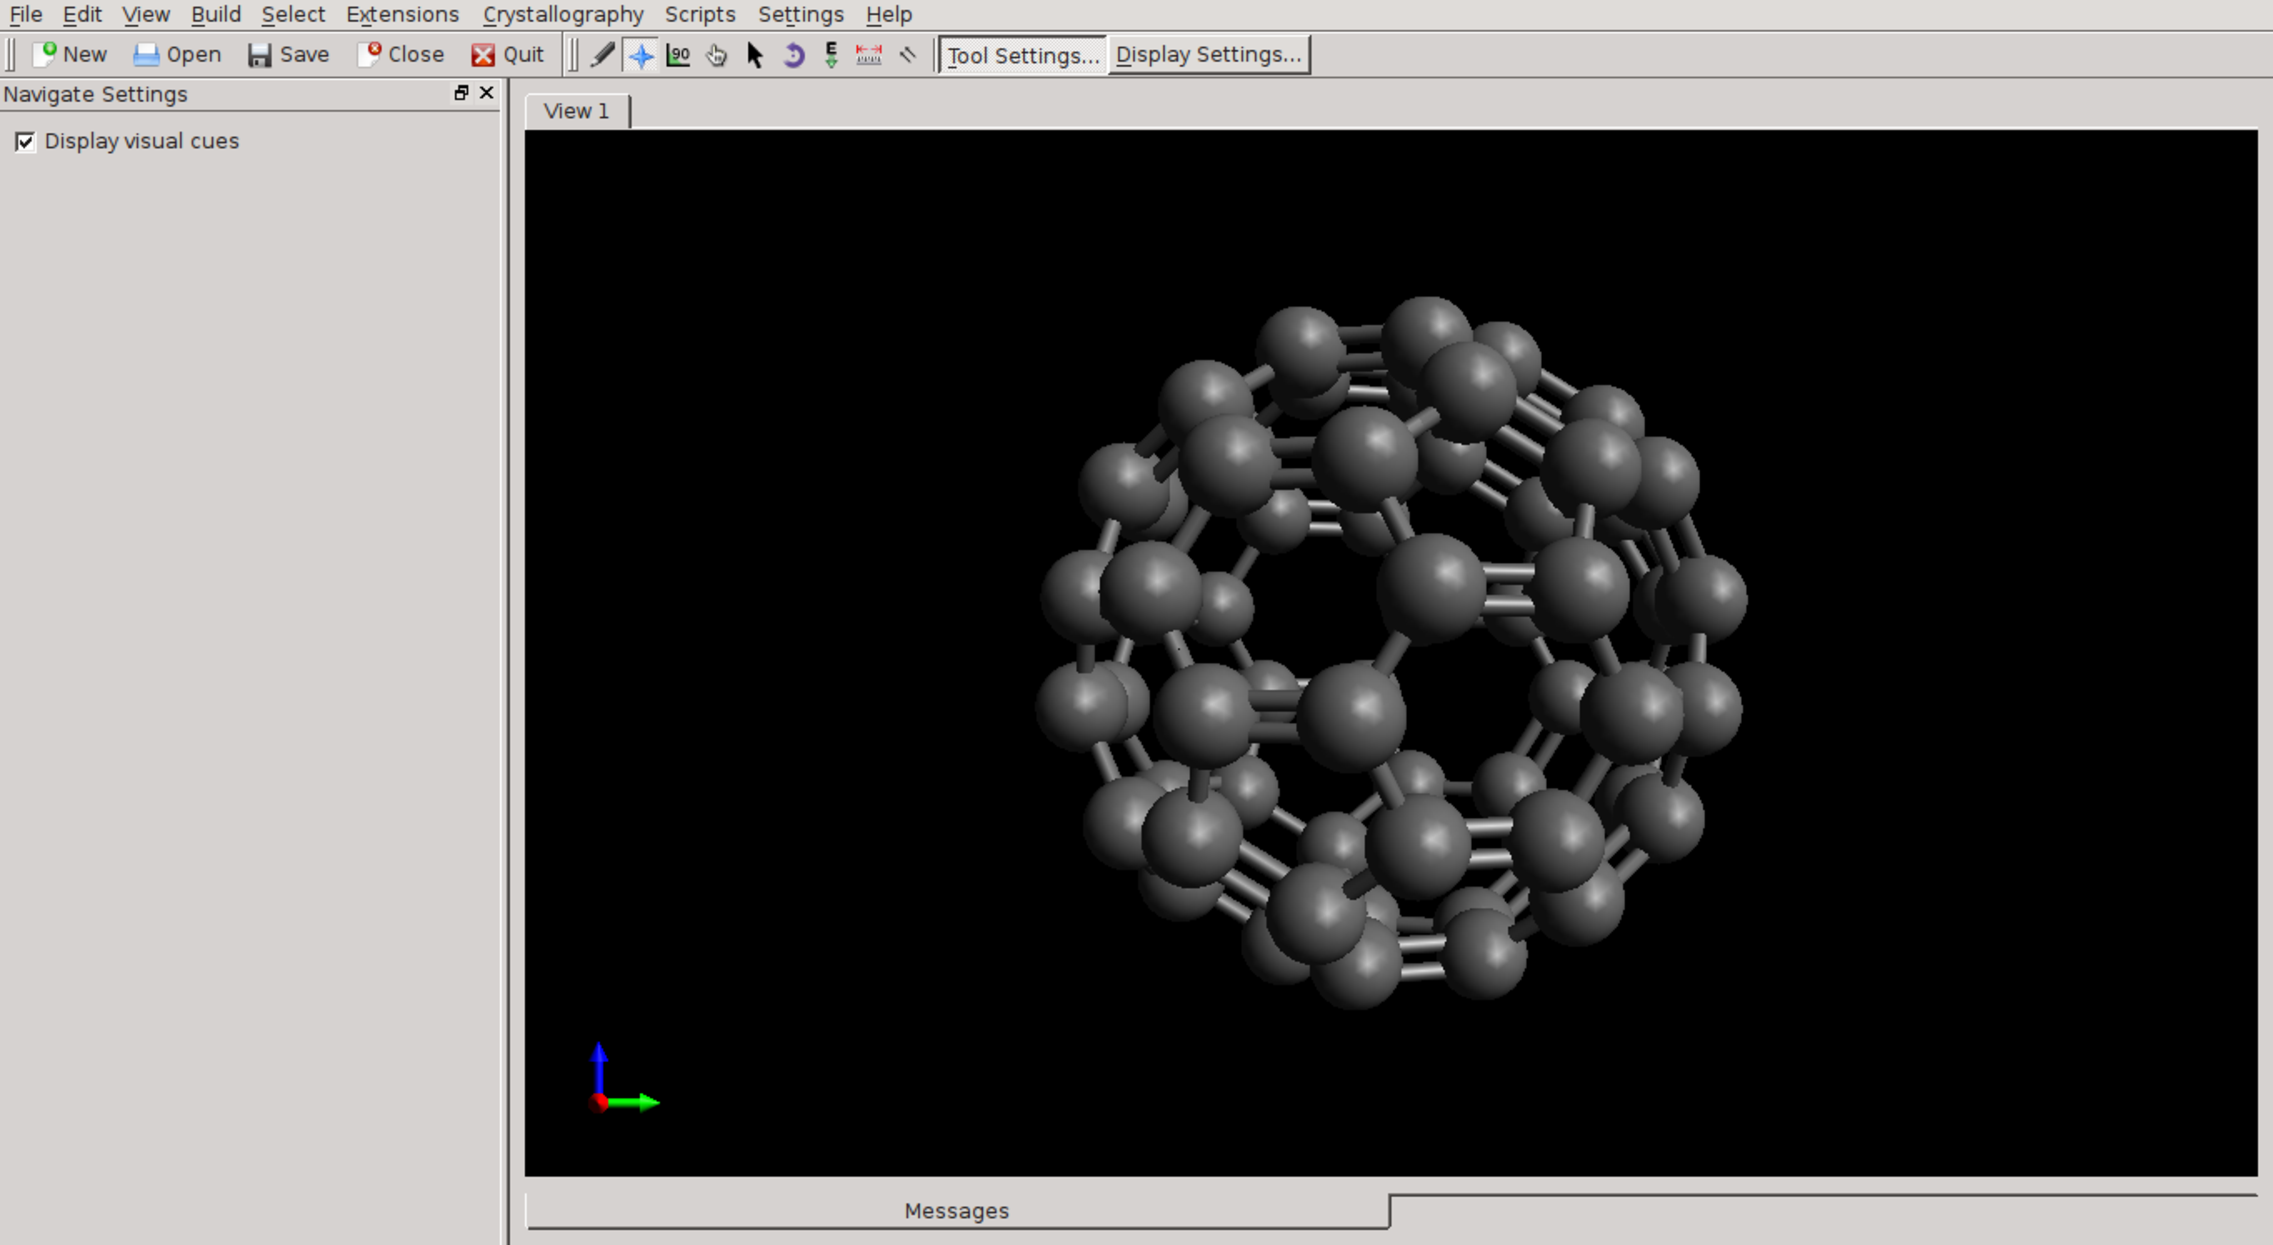
\includegraphics[width=1.0\textwidth]{./FIGs/Avogadro_screenshot.pdf}
\caption{Модель фуллерена $C_{60}$, открытая в приложении Avogadro}
\label{Avogadro_screenshot}
\end{figure}

Главным преимуществом использования формата CML для представления пространственной
конфигурации нанокластера перед использованием библиотеки DISLIN является последующее
удобство работы и редактирования этой конфигурации, используя приложение Avogadro.
Поэтому, в данной работе для визуализации получаемых пространственных конфигураций
были использованы библиотека Open Babel и приложение Avogadro.
